\section{Einleitung}
\label{sec:Einleitung}
Es können verschiedene orthopädische Erkrankungen mit einer Strahlentherapie behandelt werden.
In diesem Fall wird eine Patientin behandelt, die an \enquote{Epicondylitis ulnaris}, auch Golfellenbogen genannt, erkrankt ist.
Dabei kommt es zu Überbeanspruchung der Beugemuskulatur im Unterarm. Das führt dazu, dass es zu Rissen in den Sehnenursprüngen kommt und
somit zu Entzündungen \cite{Elle}. Durch eine Strahlentherapie werden diese Entzündungen verringert.

\section{Patientenvorstellung}
\label{sec:Vorstellung}
Seit November 2015 hat eine Patientin Beschwerden beim linken Ellenbogen. Für eine Linderung der Symptome sind eine Reihe von konservativen
Therapiemaßnahmen durchgeführt worden. Dazu gehört Ruhigstellung, Kühlung und Salbentherapie des Ellenbogens.
Diese konservativen Therapiemaßnahmen haben nicht geholfen und deshalb wird der Patientin eine Strahlentherapie des linken Ellenbogens
verordnet. Dabei wurde sie über die möglichen Wirkungen und Nebenwirkungen der Strahlentherapie durch den Arzt aufgeklärt.
Zur weiteren Diagnosen gehören eine Schilddrüsenunterfunktion und Polyarthrose.
Sie ist $\SI{168}{\centi\meter}$ groß, wiegt $\SI{78}{\kilo\gram}$ und die medialen Druckschmerzen befindet sich am linken Ellenbogen.
Durch diese Schmerzen wird ihre Bewegung auch beeinträchtigt. Für die Bestrahlung wird eine Gesamtdosis von $\SI{3}{\gray}$ verschrieben,
welche in Fraktionen von $\SI{0,5}{\gray}$ in insgesamt 6 Sitzungen appliziert werden soll. Insgesamt sollen 3 Bestrahlungen pro Woche stattfinden.
Das ist hilfreich, denn der Körper muss Zeit genug haben, auf die Behandlung zu reagieren. Falls es nach 8-10 Wochen keine Besserung ergibt,
muss die Strahlentherapie wiederholt werden.

\section{Bestrahlungsplanung}
\label{sec:Bestrahlung}
Das PTV ist in den CT-Daten bereits eingezeichnet und als nächstes wurde die Kontur des Ellenbogens als Body-Struktur eingezeichnet.
Andere Gegenstände, wie z.B. Lagerungshilfe oder Patientenliege, werden auch als Struktur eingezeichnet, weil sich diese im Strahlengang befinden können.
Dosiert wird hier auf den ICRU Referenzpunkt und das Ziel der Bestrahlungsplanung ist, dass das Planungszielvolumen durch die $\SI{95}{\percent}$
Isodosenlinie umschlossen wird. Für die Bestrahlungsplanung wurden zwei opponierende Felder mit einer
Gewichtung von 0.5 erzeugt. Die beiden Felder haben eine Größe von $\SI{12}{\centi\meter}$ x $\SI{16,5}{\centi\meter}$.
Das erste Feld hat eine Gantry-Rotation von $0^\circ$ und das zweiten eine Gantry-Rotation von $180^\circ$.
Der Bestrahlungsplan wird auf "$\SI{100}{\percent}$ target mean" normiert. Für eine Schonung des umliegenden Gewebes werden MLCs verwendet,
die an die Struktur angepasst werden können. Das ist in der Abbildung \ref{fig:kombi} zu sehen.

\begin{figure}[H]
	\centering
	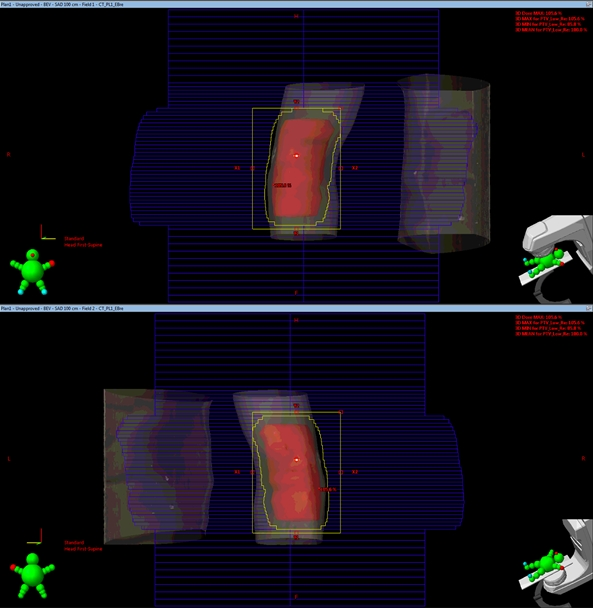
\includegraphics[width=\textwidth]{../Bilder/kombi.jpg}
	\caption{Zu sehen ist die Darstellung der Lamellen beim MLC. Beim oberen Bild handelt es sich um das Feld bei $0^\circ$ und beim unteren Bild handelt es sich um das Feld bei $180^\circ$.}
	\label{fig:kombi}
\end{figure}


\section{Auswertung und Diskussion}
\label{sec:AuswertundDiskussion}
In den Abbildungen \ref{fig:ellenbogenx}, \ref{fig:ellenbogeny} und \ref{fig:ellenbogenz} sind die Dosisverteilungen des
Ellenbogens in der Transversal-, Sagittal- und Frontalansicht zu sehen. In den Abbildungen ist zu erkennen, dass die $\SI{95}{\percent}$ Isodosenlinie
einen Großteil des rot eingezeichneten PTVs umschließt. An wenigen Stellen ist das jedoch nicht gelungen. Anhand der Dosisverteilungen ist zu
erkennen, dass die Stellen des PTVs, die nicht von der $\SI{95}{\percent}$ Isodosenlinie umschlossen werden konnten, nur knapp unterhalb der Haut liegen.
Das bedeutet, dass an diesen Stellen der Dosisaufbaueffekt stattfindet und deshalb ist es nicht möglich dort eine relative Dosis von $\SI{95}{\percent}$
zu erreichen.

\begin{figure}[H]
	\centering
	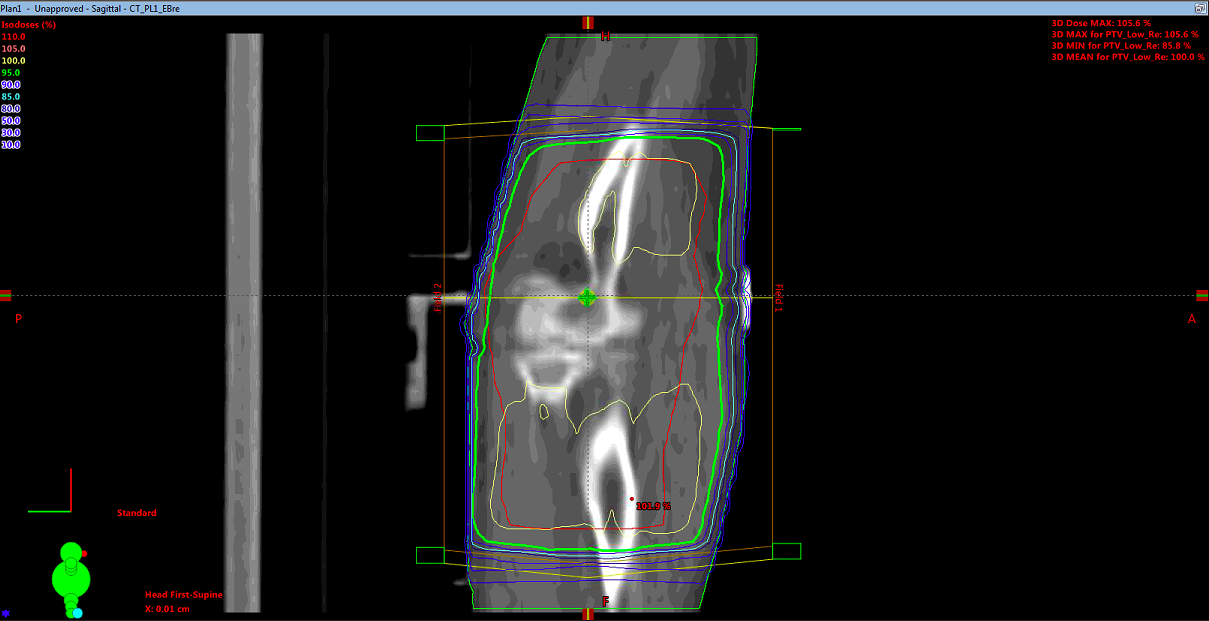
\includegraphics[width=\textwidth]{../Bilder/EllenbogenX.png}
	\caption{Darstellung der Dosisverteilung in der Sagittalansicht des Ellenbogens.}
	\label{fig:ellenbogenx}
\end{figure}

\begin{figure}[H]
	\centering
	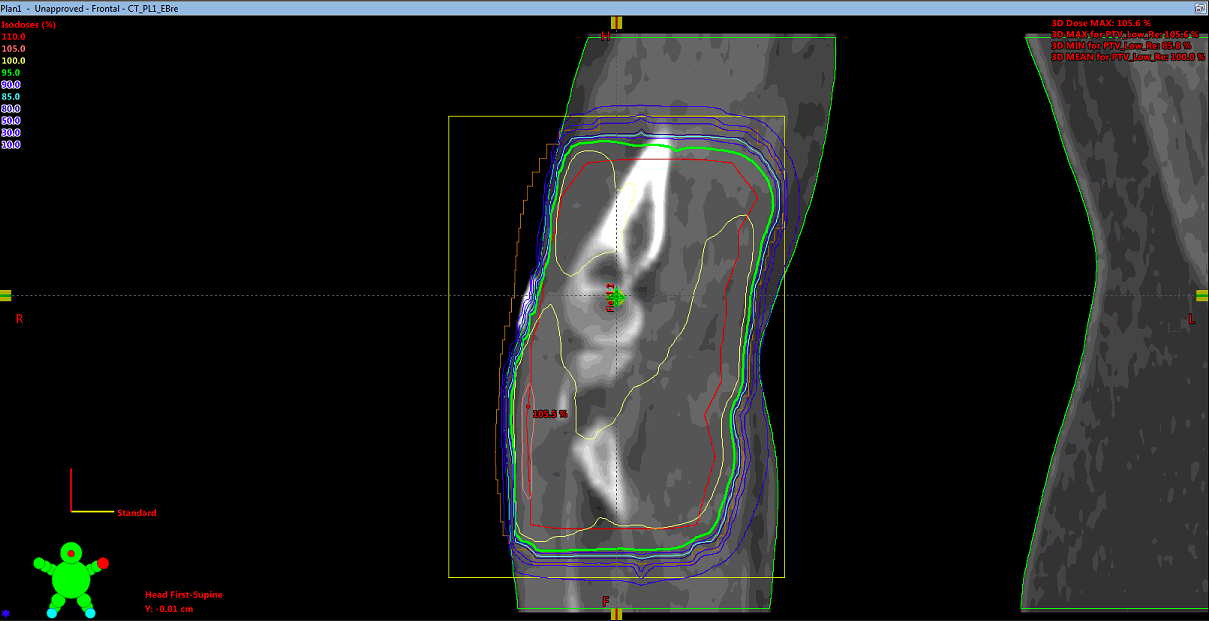
\includegraphics[width=\textwidth]{../Bilder/EllenbogenY.png}
	\caption{Darstellung der Dosisverteilung in der Frontalansicht des Ellenbogens.}
	\label{fig:ellenbogeny}
\end{figure}

\begin{figure}[H]
	\centering
	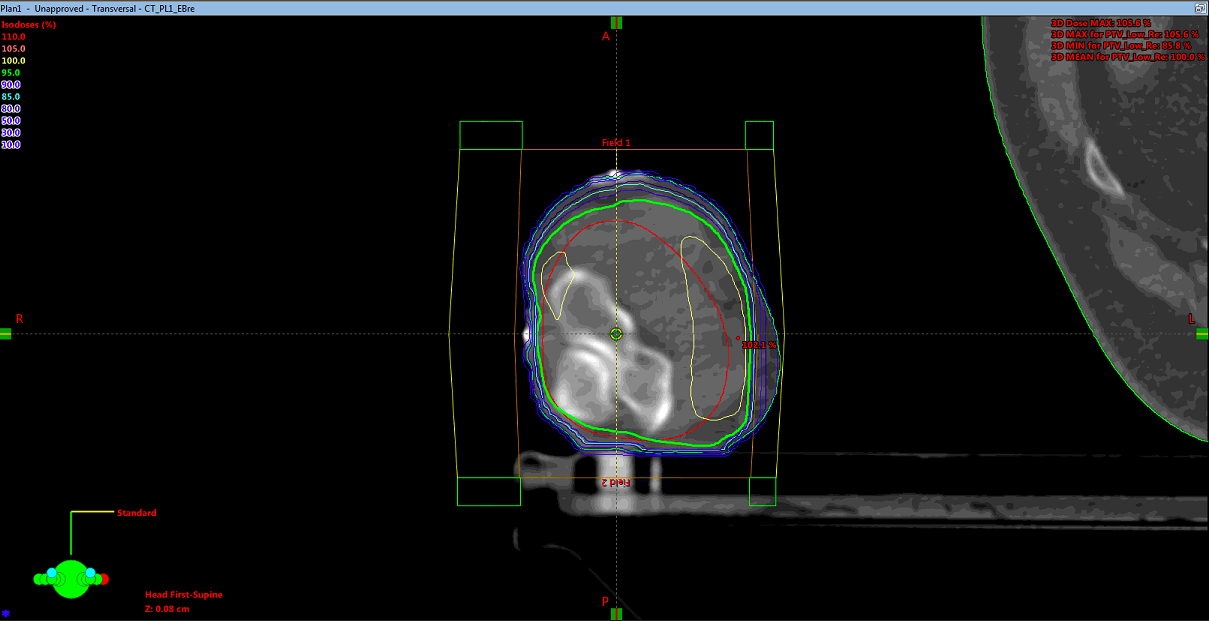
\includegraphics[width=\textwidth]{../Bilder/EllenbogenZ.png}
	\caption{Darstellung der Dosisverteilung in der Transversalansicht des Ellenbogens.}
	\label{fig:ellenbogenz}
\end{figure}

Für eine bessere Beurteilung ist das Dosis-Volumen-Histogramm in der Abbildung \ref{fig:dvhellenbogeneinzel} gezeigt.
Die maximale relative Dosis, die bis zu $\SI{107}{\percent}$ im PTV betragen darf, liegt hier bei $\SI{105,6}{\percent}$
und wurde dementsprechend eingehalten \cite{ICRU}.
Die minimale Dosis, die im PTV deponiert wird, liegt bei $\SI{85,8}{\percent}$.
Das bedeutet, dass nicht das gesamte PTV mit einer relativen Dosis von $\SI{95}{\percent}$ bestrahlt wurde.
Das konnte auch schon anhand der Dosisverteilung gesehen werden.
Nur ein sehr geringer Teil des PTVs erhält eine relative Dosis von unter $\SI{95}{\percent}$, da in $\SI{99.8}{\percent}$ des PTV Volumens
$\SI{95}{\percent}$ der Dosis deponiert wird.
Anhand des DVHs für den gesamten Arm (grüne Kurve) ist zu erkennen, dass das gesunde Gewebe gut geschützt wird.
Etwa $\SI{20}{\percent}$ des Volumens von dem Arm erhält noch eine relative Dosis von $\SI{50}{\percent}$.

\begin{figure}[H]
	\centering
	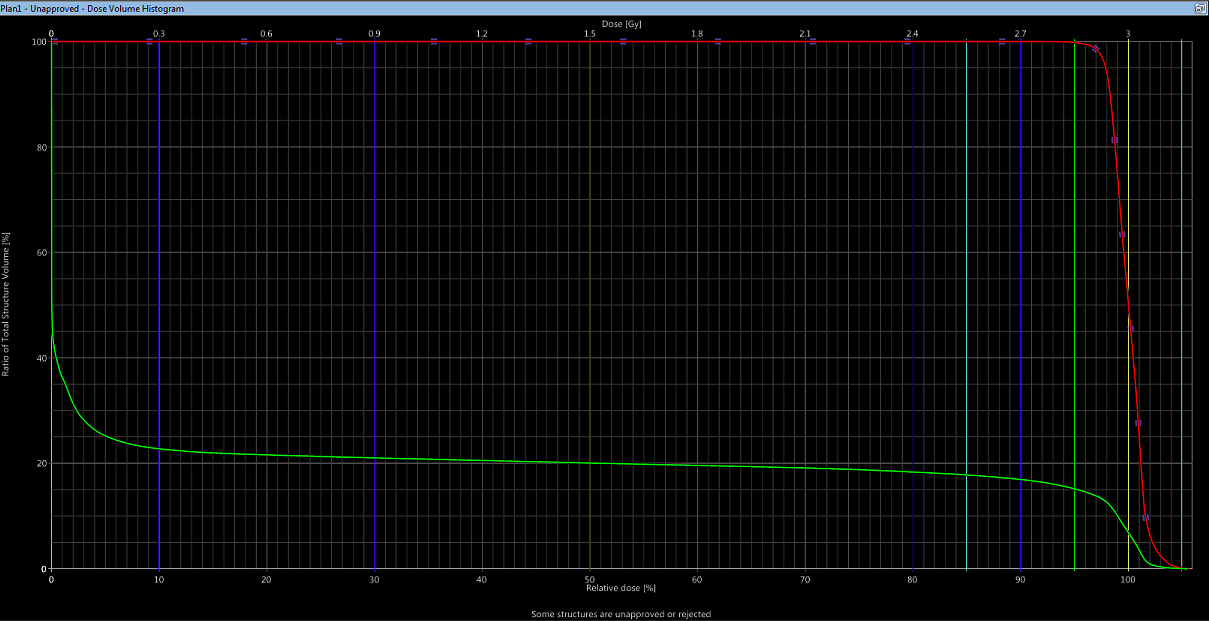
\includegraphics[width=\textwidth]{../Bilder/DVH_EllenbogenEinzel.png}
	\caption{Zu sehen ist das Dosis-Volumen-Histogramm des Ellenbogens. In roter Farbe dargestellt ist das PTV und in grüner Farbe ist das Ellenbogen. Außerdem sind noch die einzelnen Isodosenlinie eingezeichnet.}
	\label{fig:dvhellenbogeneinzel}
\end{figure}


Durch diesen Bestrahlungsplan, mit zwei opponierenden Feldern, lässt sich die gewünschte
Dosisverteilung in dem Ellenbogen gut erreichen. Nur ein sehr geringer Teil des
PTVs erhält nicht eine vorgeschriebene relative Dosis von $\SI{95}{\percent}$ und auch die
vorgeschriebene maximale Dosis wird nicht überschritten.
